\chapter{NfM}
\setcounter{section}{0}
%%%%%%%%%%%%%%%%%%%%%%%
\section{Einleitung}
\begin{center}
\textit{Eine Familie kann das Wunderbarste sein, was man je in seinem Leben erfahren wird.}	
\end{center}

Eine Familie kann das Wunderbarste sein, was man je in seinem Leben erfahren wird.

Die persönliche Erfahrung zeigt jedoch, wie anspruchsvoll es ist, eine Familie zu gründen, sie am Leben zu erhalten und gemeinsam ein schönes Leben zu führen.

Dies Strategie - \gls{p_NFM}, soll dazu dienen, diese Risiko zu minimieren, sodass eine Familie im Leben das wunderbarste sein wird.\\

Diese Strategie - \gls{p_NFM} - zielt darauf ab, dieses Risiko zu minimieren, sodass eine Familie im Leben als das Wunderbarste erlebt wird.

Die Strategie gliedert sich in:
\begin{itemize}
	\item \textit{Objectives}, welche die primären Ziele festhalten, welche wir uns für unsere Familie im Bezug zu \gls{p_NFM} setzen.
	\item \textit{\nameref{sec:Erreichung}}, die die Frage klärt, welche Ideen vorliegen, was getan werden kann oder welche Konzepte Anwendung finden, um die \glspl{p_Obj} zu erreichen.
\end{itemize}


%Um \gls{p_NFM} eine stabilie Familie zu bieten, auf welcher sie selbst später ihr eigenes Leben fußt, und für uns als Familie 

% One of the greates gift I can ofer them, is that rock, that foundation, to which build there life.

\section{Objectives} 
%NFM; Strategie Papier Name, Kategorie Name für das NFM
\subsection{Die Drei}
Die drei \gls{p_Obj} \footnote{siehe \ref{Appendix_Erlaeuterung_Objective}} unter dieser Strategie sind:

\begin{itemize}
	\item \gls{p_NFM} ist ein \underline{eigenständige} $\&$ \underline{kompetente} Mitglied in der Gesellschaft und der ganzen Familie. \label{NFM_O_1}
	% Alternative Formulierungen
	% 1 Du bist ein eig. und kompet. Mitglied in der Gesellschaft und Familie
	% 2 Wir sind veranwortlich, dass Du ein ...
	% 3 Unsere Elternrolle tragen wir verantwortungsvoll, dass Du ein eig. und kompet. Mitglied in der Gesellschaft und Familie bist.
	\item \gls{p_NFM} bekommt das Angebot, Fähigkeiten für das eigenen Leben zu erlernen. \label{NFM_O_2}
	% Alternative:
	% Strech Goal: Angebot schaffen.
	\item Die gemeinsame Zeit als Familie, gibt uns Kraft. \label{NFM_O_3}
	% Alternative Formulierungen
	% 1 Wir sind eine Familie (Keine Elternrolle), welche uns Kraft und ausnahmslose Sicherheit gibt.
\end{itemize}

Diese \gls{p_Obj} dienen zum einen der Orientierung und Ausrichtung für langfristige Entscheidungen, zum anderen sollen sie in wichtigen Momenten helfen, zu priorisieren.\\ 

Das erste \gls{p_Obj} (\nameref{NFM_O_1}) fusst auf der Überlegung, dass wir als \glspl{p_BFM} selbst eine gesellschaftliche Verantwortung haben, für die Gesellschaft keine Last zu verantworten. Im Idealfall ist \gls{p_NFM} eine Bereicherung für die Familie und Gesellschaft, mindestens keine Last. 

In unsere \gls{p_ER}, sehen wir die Erreichung als unsere Verantwortung.\footnote{
	Darüberhinaus, sehen wir auch als unsere Verantwortung, dass wir maximale Sicherheit geben. Dazu im weiteren Verlauf mehr.
}
Diese Erreichung birgt ein Risiko, welches die Erreichung von \nameref{NFM_O_3} reduziert, siehe \ref{sec:Risiko_EKB}.\\

Mit \nameref{NFO_O_3} ist gemeint, dass wir als \gls{p_FM} kontinuierlich ein schönes Leben haben können und unsere Familie eine Bereicherung für alle Mitglieder ist.\\

Zwischen \nameref{NFO_O_1} und \nameref{NFM_O_2} besteht der Unterschied darin, dass es eine Unterschied gibt, zwischen der Integrierung in die Gesellschaft und die Familie und der Auslebung des eigenen Lebens. Für das zweite \gls{p_Obj} steht im Fokus, dass wir als \gls{p_BFM} aufzeigen, welche Möglichkeiten es gibt und hin-und-wieder \gls{p_NFM} mindestens einmal über emotionale Hürden begleiten, damit \gls{p_NFM} selbst entscheidet kann, ob sie es weiterverfolgt.

\subsection{Analyse} \label{sec:Risiko_EKB}
Der folgende Abschnitt beschäftigt sich damit, welche Risiken in der Familien-Dynamik bestehen. Besonders wird der Schwerpunkt betrachtet, wie erfolgreich die gesetzten \gls{p_Obj} sich realisieren lassen und welche gegenseitigen Abhänigkeiten existieren oder im Wege stehen.\footnote{
	Wie in der näheren Erläuterung von \gls{p_Obj} beschrieben. Die gesetzten Objectives im Bezug zu \gls{p_NFM} haben kein Zeitparameter.
}

\subsubsection{Die initale Hypothese} ist, dass Entscheidungen und Maßnahmen im Zielkonflikt zwischen \nameref{NFM_O_3} und \nameref{NFM_O_1} stehen.\\

Die \gls{p_FM}, in der \gls{p_ER}, sind je nach Situation meist rechtliche, sozial, emotional und wirtschaftliche besser als \gls{p_NFM} positioniert. Dies ist nicht an und für sich kein Problem. Diese Positionierung findet auch außerhalb der Familie statt und dies damit kein alleiniges Merkmal der \gls{p_EKB}.\footnote{
	Im Zeitverlauf wird dies sich auch ändern. Die physische und damit auch kognitive Entwicklung positioniert \gls{p_NFM} besser.
}
Das \gls{p_Obj} \nameref{NFM_O_1} wird jedoch Eingriffe in das Leben von \gls{p_NFM} erfordern. Eine bessere Positionierung in den genannten Kategorien kann jedoch strategisch genutzt werden, die Eingriffe umzusetzen. Weil eine Essens von \nameref{NFM_O_1} ist, dass
\gls{p_NFM} in der Gesellschaft und im Familien-Kontext ihre Kompetenzen integrativ nutzen soll, bedeutet dies eine besser Positionierung von \gls{p_NFM} im Kontext der Familie und Gesellschaft.\\ 

\subsubsection{Conundrum} Die Annahme besteht, dass Eingriffe am besten strategisch realisiert werden\footnote{
	Wichtig: Dies ist unabhängig davon, ob das \gls{p_Obj} damit erreicht wird. Es geht nur um die Veränderung des Verhaltens von \gls{p_NFM}, nicht die interne Überzeugung.
}, wenn die \gls{p_FM} in der \gls{p_ER} besser als \gls{p_NFM} positioniert sind. Gleichzeitig sind die Eingriffe auf eine bessere Positionierung von \gls{p_NFM} ausgelegt.\\

\subsubsection{Risiken}
\begin{itemize}
	\item Ein Risiko ist, dass die Positionierung von \gls{p_NFM} trotz des \gls{p_Obj} nicht erreicht wird, weil der Wunsch besteht, diese Positionierung in der \gls{p_ER} nicht zu verlieren. 
	\item Ein anderes Risiko ist, dass der Eingriff in das eigenen Leben, in dem Fall von \gls{p_NFM}, als ungerecht und störend empfunden wird, welches widerrum \nameref{NFM_O_3} behindert.
	\item Eine argumentative Beschwichtigung oder Erläuterung mit \gls{p_NFM} kann zu gewissen Zeitpunkten in der physischen Entwicklung nur eingeschränkt möglich sein.
\end{itemize}

Unter Betrachtung dieser Risikoanalyse, wird im nächsten Abschnitt adressiert, wie die \gls{p_Obj} unter der Betrachtung der Risiken erreicht werden können.
% Optional Glossar: Eingriffe

Wie mit diesen Risiken umgegangen werden soll, wird im nächsten Abschnitt behandelt.

\section{Erreichung}\label{sec:Erreichung}
% Experimenten Kiste
% Maßnahmen
% Strategische Pillars
% Ideen Pool
% Stratigice Action
% Erreichung


Um die drei \glspl{p_Obj} zu erreichen wird im Folgenden ausgeführt, welche ersten Konzepte oder Maßnahmen ergriffen werden, um sie auszutesten.\\

Hierbei handelt es sich, um bisherige Ideen, welche jetzt in den kohärenten Rahmen von \gls{p_NFM} gebracht werden. Nicht alle bisherigen Ideen werden für den ersten Entwurf hier integriert werden, weil sie entweder nicht weit genug zu ende gedacht sind oder nicht mit den Zielsetzungen vereinbar sind oder die Zeit nicht ausreicht, sich mit alle vorherigen Gedanken intensive auseinander zu setzen. Themen, welche sich nicht mit \gls{p_NFM} vereinigen lassen aber dennoch sinnvoll sind diese schriftlich auszudenken, werden im Abschnitt \ref{subsec_MissFits} ausgeführt.\\
% Weitere Ideen sind in den Notizen festgehalten.


Nicht alle hier beschriebenen Maßnahmen oder Ansätzen werden erfolgreich umgesetzt oder erbringen den erhofften Erfolg. %Alle Abschnitte haben jedoch eins gleich, sie setzten sich mit den \gls{p_Obj} und Risiken auseinander und streben so ein koheräntes Vorgehen an.
Der Funktion\footnote{
	Synonym: algorithmisches Vorgehen/ strategisches Denken
} dieses Abschnittes ist jedoch, sich im Vorfeld, wie eine genaue Erreichung der \gls{p_Obj} angegangen werden kann, wie diese mit anderen Aktionen im Einklang oder nicht im Einklang ist. Welche Annahmen liegen zugrunde, warum eine gewisse Aktion oder Konzept zu der Erreichung der \gls{p_Obj} führt.\footnote{
	Nicht immer wird die im Detail hier ausgeführt. Es ist aber unabdingbar, diese Gedanken sich zu machen und ein kohärentes Bild von der Maßnahme und dem Konzept aufzuzeigen.
}\\

Ebenso werden einig dieser Maßnahmen und Konzept sich im Zeitverlauf entwickeln, weil neue Ideen entsprungen sind, wie ein erfolgreicherer Ansatz gestaltet werden kann oder neue Erkenntnisse aus dem ausprobieren hervorgegangen sind. Ein kontinuierliches schriftliches Update dieser ist erstmal nicht vorgesehen.\footnote{
	Das algorithmische Vorgehen, wie Maßnahmen und Konzept sich kohärent in \gls{p_NFM} integriert lassen, bleibt weiter der mentale Anspruch.
}
%TODO: In den Notizen sind erstmal unstrategisierte Gedanken nieder geschrieben. Diese können genau auf die Zielsetzung einzahlen oder nicht. Es gibt somit mehr Idee als hier beschrieben.

\subsection{Reduzierung in der Relevance der Elternrolle -\gls{p_RiRER}}

Eine Prinzip was besonders in den ersten 18 Jahren der \gls{p_EKB} Anwendung finden wird, ist  \gls{p_RiRER}.\\
% Was es mit dem Risiko zu tun hat, wird später erläutert.

Um dies zu erreichen, werden drei Kategorien: 
\begin{itemize}
	\item Entscheidungen,
	\item Ressourcen
	\item und Betreuung
\end{itemize}\footnote{
	Hierbei sind Entscheidungen gemeint, welche direkt oder indirekt für \gls{p_NFM} getroffen werden; Besonders finanzielle und soziale Netzwerk-Ressourcen besitzt \gls{p_NFM} zum Start noch nicht; Nicht alle Unterfangen kann \gls{p_NFM} selbstständig angehen. Meist Bedarf es Fähigkeiten eine gewisses Unterfangen durchzuführen. Selbst wenn das Unterfangen selbst von \gls{p_NFM} durchgeführt werden kann, die anderen Fähigkeiten nicht.
}
betrachtet.
\subsubsection{Transit}
Bei diesen Kategorien soll ein Transit erfolgen, welche die \gls{p_RiRER} reduziert und somit auf \nameref{NFM_O_1} einzahlt. Der Verlauf wird nicht linear erfolgen, jedoch durch die kontinuierliche Übergabe von Verantwortung, Vermittlung von Kompetenzen, Reduktion von beeinflussender Entscheidungen \gls{p_NFM}s Leben, soll so sichergestellt werden, dass \nameref{NFM_O_1} kontinuierlich überprüft werden kann, wie erfolgreich sich \gls{p_RiRER} auswirkt. 

Wir antizipieren, dass an gewiesen Abschnitte im Leben von \gls{p_NFM}, dass die Relevanz für die \gls{p_ER} wieder ansteigen wird, um entweder gesellschaftlichen Hürden zu überwinden oder physische Entwicklungsschritt abzufädern, wenn sie sich negativ auf \nameref{NFM_O_1} oder \nameref{NFM_O_3} auswirken.

\begin{figure}[H]
	\centering
	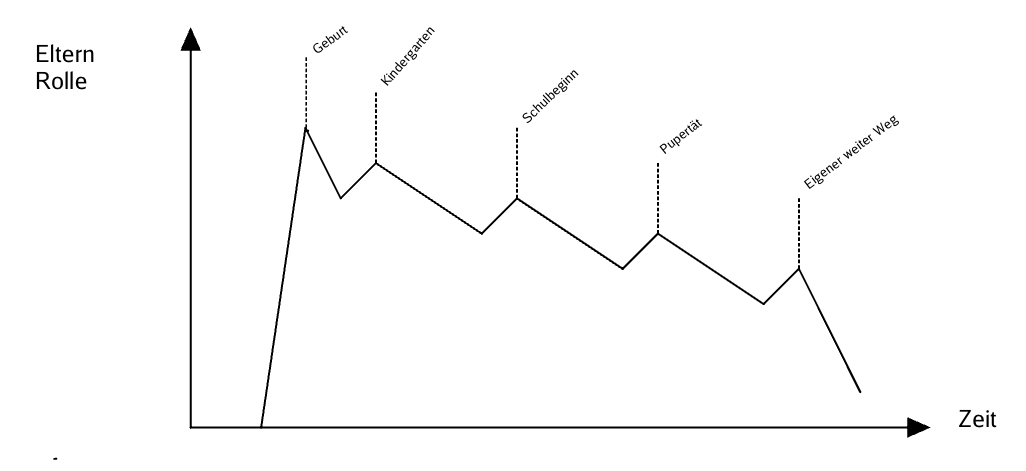
\includegraphics[scale = 0.3]{attachment/chapter_OWN/Scc005.png}
	\caption{Versinnbildlichung der Relevanz der \gls{p_ER} im Zeitverlauf}
\end{figure} 

\subsubsection{Raum zur Debatte} Wie weit der Transit vollzogen ist, wie weit die drei \gls{p_Obj} vorangeschritten sind, wird sich nicht eindeutig bestimmen lassen oder von allen gleich aufgefasst. Um dies als Familie \textit{permanent} auszuloten, benötigt es \underline{Raum zur Debatte}. Vorallem für \gls{p_NFM} sehen wir es als wichtig an, dass der Raum gegeben wird
\begin{itemize}
	\item unser Annahmen, Schlussfolgerungen und angeleiteten Maßnahmen herausgefordern, 
	\item eigenen Themen einbringen zu können
	\item und gemeinschaftlich über den aktuellen Status zu reflextieren.
\end{itemize}



\subsection{Umgang mit Geld}
Mit Abnahme der \gls{p_RiRER} geht einher, dass \gls{p_NFM} mehr Verantwortung in der Familie und Gesellschaft bekommt.\\

Der Umgang mit Geld ist ein Standbein, welcher dabei hilft, eine Reduktion bei den Ressourcen zu kompensieren. Ein möglicher Ansatz ist, dass \gls{p_NFM} ein eigenes gemeinsames Konto bekommt. Auf diesen zahlen wird für es eingezahlt, alle Ausgaben für \gls{p_NFM} werden darüber getätigt. Ab einen gewissen Zeitpunkt, bekommt \gls{p_NFM} selbst Zugang zu diesem Konto, von welchem es die eigen Sachen bezahlen kann. Die Fähigkeit, welche \gls{p_NFM} dabei erlangen soll, ist mit limitieren Ressourcen umzugehen. Anderes, als wenn die \gls{p_NFM} die \gls{p_FM} fragt, und diese es zahlen.\footnote{
	Hierbei gibt es keine limitierte Ressource, weil die \gls{p_FM} immer gefragt werden kann.
} Die \gls{p_FM} helfen vor allem im ersten Prozess. \footnote{
	Zusätzlich kann hierbei Plus und Minus schon gelernt werden.
}


\subsection{Wissenskatalog}
\subsubsection{Zielsetzung}
% Alternativen: In in den Epolog zu stecken.
% Andere Formulierung: Es geht darum, anzustreben, welche Einschränkungen bei NFM vorliegen.
Die nächste Abschnitt beschäftig sich damit, welche physischen Merkmale in der Entwicklung von \gls{p_NFM} zu berücksichtigen sind.\\ 

Das Ziel diese Wissenskatalog ist, dass \gls{p_tpR} bei der Erreichung der \gls{p_Obj} oder Umsetzung der anderen \ref{sec:StrategischePillars} mit einfaktoriert sind. Zum Beispiel bei der \gls{p_RiRER} sollen die \gls{p_tpR} dabei unterstützen, Erwartungen richtig zu setzen und Reduktionen der Elternrolle anzustreben, wenn es am plausibelsten ist.\\

Das Ziel ist, dass \gls{p_NFM} besser in ihrer physischen Entwicklung verstanden wird, sodass bei \gls{p_RiRER}, die eigenen Erwartungen 
bei gegeben Maßnahmen zu einer erfolgreicheren Erreichung von \nameref{NFM_0_1} ohne \nameref{NFM_0_3}
das richtige Maß an Reduktion zur richtie 


Im Folgenden werden \gls{p_tpR} lose aufgegriffen. Einige werden dabei direkt mit einfaktoriert werden können und andere werden sich indirekt im Verhalten berücksichtigt werden lassen.\\
	
\subsubsection{Zeitverlauf}
\begin{enumerate}%[align=left,leftmargin=*,widest=10]
	\item[Geburt]
	\begin{itemize}
		\item Erster Atemzug: Zur Geburt wird durch einen Adrenalienschub die ungenutzten Lungen zur Atmung animiert.
		\item Muskeln Kontraktion: Muskeln müssen erste jetzt komplett die Funktion übernehmen.
		\item Herz: Dies hat zwei Löcher. Diese schließen sich in den ersten Tagen. Grund dafür ist, dass die Lungen jetzt mit Blut versorgt werden müssen, welches sie vorher nicht mussten.
		\item Erster Stuhlgang: Dieser besteht aus einer grünen Flüssigkeit, welcher sich aus der Verdauungsflüssigkeit ohne jegliche Nahrung besteht.
	\end{itemize}
	\item[1 Woche]
	\begin{itemize}
		\item Temperatur
		\begin{itemize}
			\item Körper von \gls{p_NFM} muss sich an eine neue Außentemperatur anpassen. Es kommt zu einem Temperaturabsturz von \SI{38}{\celsius} zu durchschnittlich \SI{18}{\celsius}.
			\item Der Hypothalamus ist bei neu geborenen nicht vollständig entwickelt, eine eigene Temperaturregulierung ist noch nicht möglich.
			\item Zusätzlich besitzen \gls{p_NFM} eine große Körperoberfläche im Verhältnis zum Körpervolumen. Dies verursachte einen hohen Temperaturverlust. 
			\item Gewinnung von Wärme aus Muskelkontratkion ist im ersten Jahr nicht möglich.
			\item Die Wärmentwicklung wird durch Braunefettzellen gesteuert. Diese Wärmequelle nimmt im ersten Lebensjahr ab, bis der Körper eigenständig die Wärmeregulierung übernehmen kann.
			\begin{figure}[H]
				\centering
				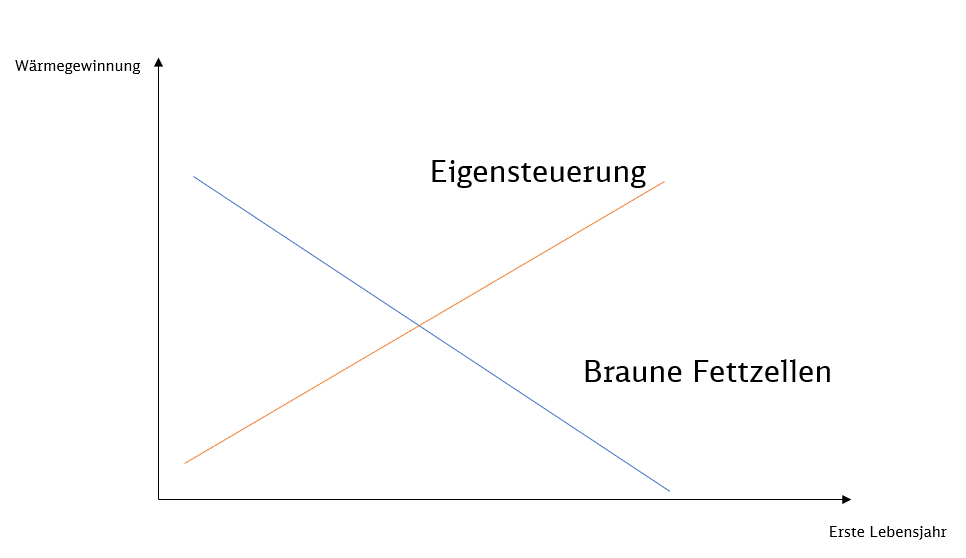
\includegraphics[scale = 0.3]{attachment/chapter_9/Scc001}
			\end{figure} 
		\end{itemize} \footnote{Empfehlung: Generell fühlen sich Säuglinge gut angezogen bei einer Raumtemperatur von etwa 24 bis 25 Grad Celsius am wohlsten. Herrschen aber in den Räumen der Wohnung „normale“ Temperaturen, das heißt zwischen 20 und 23 Grad Celsius im Wohnzimmer und 17 bis 20 Grad im Schlafzimmer, sind ein Body oder ein Shirt aus Baumwolle genau das Richtige zum Unterziehen für das Baby. Darüber eignet sich dann ein recht enganliegender leichter Pullover, beziehungsweise ein nicht allzu dickes Sweatshirt optimal.}
		\item Immunsystem
		\begin{itemize}
			\item Das Immunsystem wird bis das Stillen abgeschlossen ist, von der Muttermilch unterstützt. Antikörper werden über die Milch übertragen.
			\item Gleichzeitig trägt der enge Bund dazu bei, dass die Mutter den gleichen Erregern ausgesetzt ist.
		\end{itemize}
		\item Plötzlicher Kindstod
		\begin{itemize}
			\item Genaue physische Ursachen sind für dieses Phanomän sind nicht ableitbar.
			\item Empfehlungen wie: \textit{Säuglinge} im ersten Lebensjahr sollen immer auf dem Rücken einschlafen, und es soll kontrolliert werden, dass dies auch durch die Nacht hin passiert. Es ist dabei möglich, dass auf dem Bauch zuerst eingeschlafen wird und später der Säugling umgedreht wird. 
			\item Tagsüber ist für die Ausbildung der Rückenmuskulatur entscheidend, dass der Säugling auf dem Bauch liegt. 
		\end{itemize}
	\end{itemize}
	\item[6 Wochen]
	\begin{itemize}
		\item Iterationen mit unvertrauten Umgebungen sind eine hohe Lernherausforderung. Beispiel: Ein Besuch im Supermarkt zählt zu solchen Lerneindrücken.
		\item Die Hörqualität wird mit weiterem Alter nur noch abnehmen, und ist somit nie wieder so gut, wie als Neugeborenes.
		\item Retina und die Muskulatur zum Einstellen der Linse ist noch nicht entwickelt und trainiert. Diese führt dazu, dass schwarz-weiß und unscharf gesehen wird.
		\item Nach ca. 2 Monaten können Farben auseinander gehalten werden.
		\item Nach ca. 4 Monaten können Gesichter auseinander gehalten werden.
		\item In den ersten drei Monaten herrscht eine Wachstumsrate von 25 $\%$ je Monat
		\item Ab 6 Monaten kann sich ein Säugling meist drehen. Dies erhöht das Risiko für einen plötzlichen Kindstod.
	\end{itemize}
	\item[8 Monate]
	\begin{itemize}
		\item Alle Sinne sind vollständig ausgebildet.
		\item Mit dem Tastsinn werden weitere Lernprozesse angestoßen.
		\item Weil die Dichte im Mund an Sinneszellen sehr hoch ist, wird dieser genutzt, um eine höhere Lernqualität zu erhalten. Der Mund besitzt spezielle Enzyme, welche Bakterien angreifen.
		\item Mit dem 9 Lebensmonat startet die Aushärtung der Kopfform und Knochenbildung. Dies führt dazu, dass Asymetrien sich ab diesen Zeitpunkt verfestigen. Bis zum Ende des ersten Jahres ist dieser Prozess abgeschlossen.
	\end{itemize}
	\item[1 Jahr]
	\begin{itemize}
		\item Durch die Möglichkeit des Krabbels startet die Entwicklung von einem Baby zu einem Kleinkind.
		\item Fähigkeit des Sprechens wird entwickelt
	\end{itemize}
	\item[11 Jahre]
	\begin{itemize}
		\item Hormonbildung startet.
		\item Die sexuelle Entwicklung startet.
	\end{itemize}
\end{enumerate}
\footnote{
	Quelle 1: \href{https://www.ipzf.de/gehirnentwicklung.html}{Link},
	Quelle 2: \href{https://www.youtube.com/watch?v=ZNYv_ory8rc}{Living Body Documentation},
	Quelle 3: %\href{https://kinderzeit-bremen.de/familienzeit/schwanger-und-baby/waermehaushalt-bei-neugeborenen-tipps-risiken/#:~:text=Gerade\%20in\%20den\%20ersten\%20neun,kommt\%20es\%20rasch\%20zu\%20Temperaturverlust.}{Wärmehaushalt bei Neugeborenen}
	%Quelle 4: \href{https://www.varilag.de/ratgeber/baby-kopfform/#:~:text=Die\%20Sch\%C3\%A4delbasis\%20entwickelt\%20sich\%20aus,die\%20den\%20Sch\%C3\%A4del\%20flexibel\%20halten.}{Die Kopfform von Babys}
}






\subsection{Batterien Aufladen}

Um den \textit{Akku} jedes \gls{p_FM} aufzuladen, benötigt es Zeit, in welcher jeder frei von Verantwortung ist oder die Dinge tuen kann, welche die Energie Reserven wieder auffüllen.\\

Die hier beschriebene Maßnahme ist recht simple. Die \gls{p_BFM} haben die Verantwortung und Pflicht auf sich selbst zu achten, dass sie Kraft, Gedult und kongnitiv nicht eingeschänkt sind. Dies ist unabdingbar, wenn 

Eine Verantwortung kann sein, 
- dass Erwartungsbilder an einen gestellt werden und diese durch die physische Nähe als bewusst oder unbewusst von einem selbst als Verantwortung gespürt werden. Eine physische Entkopplung von Personen ist daher notwendig, um eine bewusst oder unbewusste Anpassung des eigenes Verhaltens zu verhindern. Denn diese benötigt Energie, um sie zu realisieren. Z.B.: Eine Erwartungsbild wird meist hervorgerufen, von allen Personen, bei welchem man keine vollständige Sicherheit verspürt. Dies wären Franziska. Die eigene Familie wäre dies auch, wenn ein Form von Alltag vorherrscht. Den wenn dieser nicht vorherrscht, besteht das Erwartungsbild zum Beispiel, dass man was unternehmen will/ Zeit maximieren möchten.
- Passive Tätigkeiten. Tätigkeiten, welche ebenso eine Teil-Aufmerksamkeit erfordern, haben zwar keinen großen Einfluss auf den Energie-Haushalt, sie tragen aber nicht dazu bei das der „Akku“ sich wieder auflädt. Sie verbrauchen ihn nur nicht so stark.

Eine Erholung entsteht, wenn keine Verantwortung vorherrscht. Aufgaben, in welchen man selbst keine Verantwortung für andere spürt, können somit ebenso als Erholung verstanden werden. 

Sinnvolle Investition aber Trotzdem Akku Verbrauch

Es ist jedoch zu berücksichtigen, dass mentale oder physische Tätigkeiten, welche kein Verantwortung gegenüber anderen Personen erfordern, trotzdem eine eine Energie-Investition darstellen. Neue soziale Interaktionen erfordern eine Aufmerksamkeit. Diese Interaktionen können routiniert wirken, können jedoch trotzdem Aufmerksamkeit erfordern. Zum Beispiel: Weihnachten bei der Familie. Diese Zusammenkommen kann einem ähnlichen Verlauf folgen. Neue soziale Dynamiken können jedoch Aufmerksamkeit erfordern. 

Bekannte und kommende Tätigkeiten kommunizieren

Bestimmt Tätigkeiten, welche schon bekannt sich, welche einem helfen, Energie zu tanken, sollten gut kommutiert werden, damit diese auch erkannt werden, dass genau diese zu einer Stärkung des Partners führen. Besonders für neue Tätigkeiten sollten kommuniziert werden, damit auch diese erkannt werden.


